\documentclass[10pt,a4paper,twoside]{article}
\usepackage[a4paper,top=20mm,bottom=20mm,outer=5cm]{geometry}
\usepackage[utf8]{inputenc}
\usepackage[english]{babel}
\usepackage{graphicx}
\usepackage{hyperref}
\usepackage{amsmath}
\usepackage{acronym}
\usepackage{cleveref}
\usepackage{natbib}
\bibliographystyle{abbrvnat}
\setcitestyle{authoryear}


\title{Project Machine Learning\\--- Milestone 1 ---} 

%%%%%%%%%%%%%%%%%%%%%%%%%%%%%%%%%%%%%%%
%                                     %
%   EVERYTHING BELOW CAN BE CHANGED   %
%                                     %
%%%%%%%%%%%%%%%%%%%%%%%%%%%%%%%%%%%%%%%

\author{Konstantin Ausborn, Timon Palm, Marco Rosinus Serrano}
\date{\today}

\begin{document}
\acrodef{ae}[AE]{Autoencoder}
\acrodef{vae}[VAE]{Variational Autoencoder}
\acrodef{vq}[VQ-VAE]{Vector Quantized Variatonal Autoencoder}
\acrodef{gan}[GAN]{Generative Adversarial Networks}
\acrodef{dnn}[DNN]{Deep Neural Networks}

\maketitle

We need to state our focus on images before this section begins.

\section{Baseline method and evaluation}\label{sec:baseline-method-and-evaluation}
The \ac{vq} described in the paper fulfills two tasks.
The first is learning useful and compact, discrete representations of real world data, the second generating new samples
in this representation space and decoding them back to the original data space.
The paper mainly focuses on the generative aspect, but to understand the whole model better, we want to gain insights
into both, and chose our baseline methods accordingly.

\subsection{Baselines}\label{subsec:baselines}
While there exist multiple machine learning approaches with a setup similar to that of the \ac{vq}
i.e.\ generative models with latent representations such as \ac{gan}, differences in the details make these hard to
compare against each other.
When sticking to the example of \ac{gan}, one key difference is that in the basic model, the latents can not be created
by encoding real world data but overall represent a distribution that is close to that of the training data~\cite{gan}.

Another requirement for or baseline model is some simplicity.
Since it is the original model that the non-quantized \ac{vae} is based on, which in turn later was developed into the
\ac{vq} and because it also fulfils the requirement of simplicity, we chose the basic \ac{ae} as our general baseline
method.
We also incorporate some experiments with the \ac{vae}, to show the progress that was made over time.

The similar architecture of these baselines allow for very comparable results, since they can be tuned to be very
close in size, training cost and latent structure.

While much of the current work in realistic high resolution image generation is based on \ac{dnn} \cite{addsources},
the field of image compression is well researched both in-, and outside deep architectures~\cite{compression},
and non-ML approaches are still dominant on the web~\cite{img_file_format}.
To represent this, we also use the popular JPEG format for comparisons against our lossy compression schemes.

\begin{figure}[h]
    \centering
    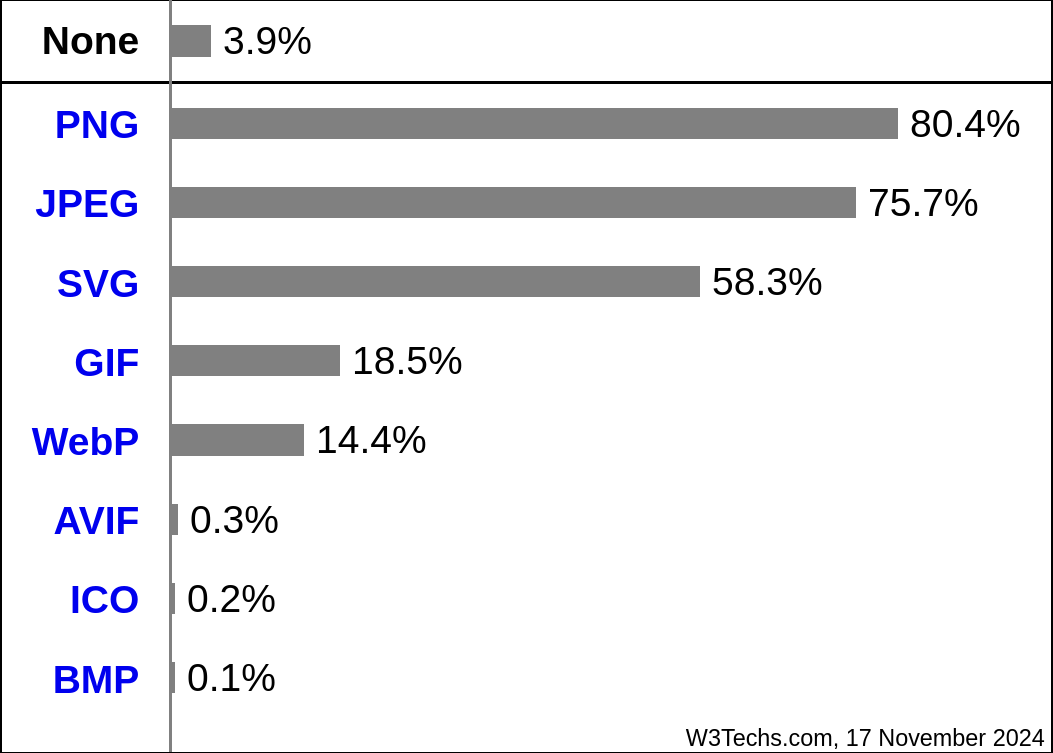
\includegraphics[width=0.5\textwidth]{images/formats}
    \caption{Percentages of websites using various image file formats. Note that a website may use more than one image file format~\cite{img_file_format}}
    \label{fig:file_formats}
\end{figure}

\subsection{Evaluation Metrics}\label{subsec:evaluation-metrics}
\subsubsection{Compression}
bits per pixel for compression rate
ssim
\subsubsection{Image Generation}
Marginal NLL or NLE, basically just use negative log entropy as the factor to compare, this describes the entropy of the picture generated?

\begin{itemize}
    \item I do not have clarity here see: https://bjlkeng.io/posts/a-note-on-using-log-likelihood-for-generative-models/
    \item I need to understand PixelCNN better to continue
    \item see Shannon for theory on entropy\cite{shannon}
    \item dont use parzen windows\cite{note_on_eval}
    \item
    \item
\end{itemize}

\section{Discussion}
:-)

\bibliography{bibliography}
\end{document}
